%!TEX program = xelatex
\documentclass[cn,hazy,blue,14pt,screen,device=normal]{elegantnote}
\usepackage{multirow}
\usepackage{enumitem}
\usepackage{caption}
\usepackage{tabularx}

\title{物理层提供的服务}

\author{李聪聪}
\institute{3GPP TS 38.202 V15.6.0}

\version{0.4}
\date{\zhtoday}

\usepackage{array}

\begin{document}

\maketitle

\newpage
\tableofcontents
\newpage

\section{物理层的服务和功能}
\subsection{概述}
高层通过使用 MAC 层与物理层之间的传输信道来使用物理层所提供的数据传输功能。所谓传输块(Transport Block, TB),即 MAC 层与物理层之间传输的数据。

\subsection{L1 功能概述}
为了实现数据传输服务,物理层需要具备以下功能:
\begin{itemize}[leftmargin=2cm]
	\item 传输信道的错误检测并向高层指示
	\item 传输信道的向前纠错(FEC)编码/解码
	\item 混合自动重传请求(HARQ)软合并
	\item 编码的传输信道与物理信道间速率匹配
	\item 将编码的传输信道映射到物理信道上
	\item 物理信道的功率加权
	\item 物理信道的调制与解调
	\item 频率和时间同步
	\item 无线电特性测量和对高层的指示
	\item 多入多出(MIMO)天线处理
	\item 射频处理
\end{itemize}

\section{UE 的物理层模型}
所谓 5G-NR 物理层模型,即指从更高层的角度来看的相关 5G-NR 物理层的特征。具体包括以下内容:
\begin{itemize}[leftmargin=2cm]
	\item 从物理层向上或向下传递的高层数据的结构
	\item 高层可以用来配置物理层的方法
	\item 物理层提供给高层的不同指示(错误指示、信道质量指示等)
\end{itemize}

\subsection{上行模型}
\subsubsection{上行共享信道}
上行共享信道(UpLink Shared CHannel, UL-SCH)传输的物理层模型如图 \ref{PhysicalLayerModelForULSCHTransmission} 所示。图中蓝色部分显示的处理步骤表示它们可以通过高层配置。
\begin{figure}[!htbp]
	\centering
	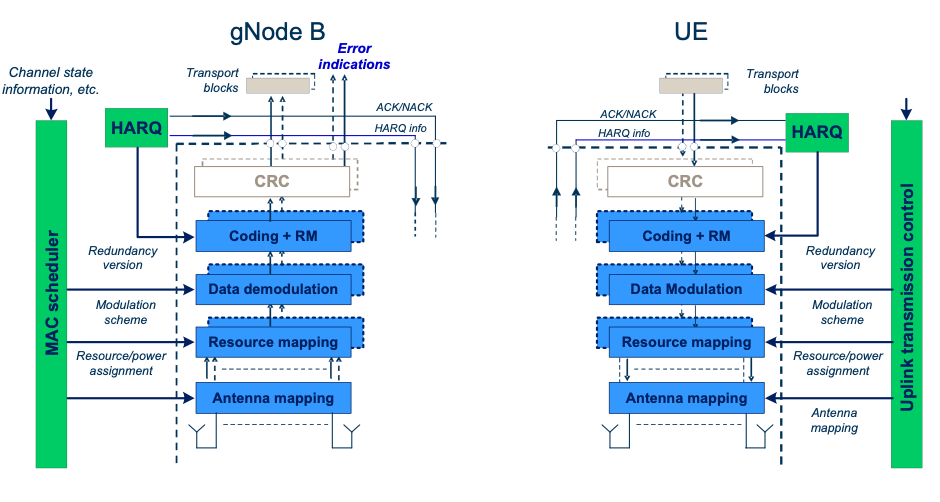
\includegraphics{PhysicalLayerModelForULSCHTransmission}
	\caption{上行共享信道传输的物理层模型}
	\label{PhysicalLayerModelForULSCHTransmission}
\end{figure}

该模型中包括以下步骤:
\begin{itemize}[leftmargin=2cm]
	\item 传递到物理层或从物理层传递的高层数据
	\item CRC 和传输块错误指示
	\item 向前纠错编码和速率匹配
	\item 数据调制
	\item 物理资源映射
	\item 多天线处理
	\item 支持 L1 控制和 HARQ 相关的信令
\end{itemize}

\subsubsection{随机接入信道}
用于随机接入信道(Random Access CHannel, RACH)传输的物理层模型的特征在于 PRACH 前导格式。如图 \ref{PrachPreambleFormat} 所示,该格式由循环前缀、前导码和保护时间组成。在此期间,不会传输任何信息。

\begin{figure}[!htbp]
	\centering
	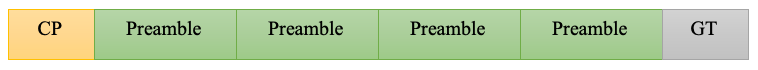
\includegraphics{PrachPreambleFormat}
	\caption{PRACH 前导格式}
	\label{PrachPreambleFormat}
\end{figure}

\subsection{下行模型}
\subsubsection{下行共享信道}
下行共享信道(DownLink Shared CHannel, DL-SCH)传输的物理层模型如图 \ref{PhysicalLayerModelForDLSCHTransmission} 所示。图中蓝色部分显示的处理步骤表示它们可以通过高层配置。
\begin{figure}[!htbp]
	\centering
	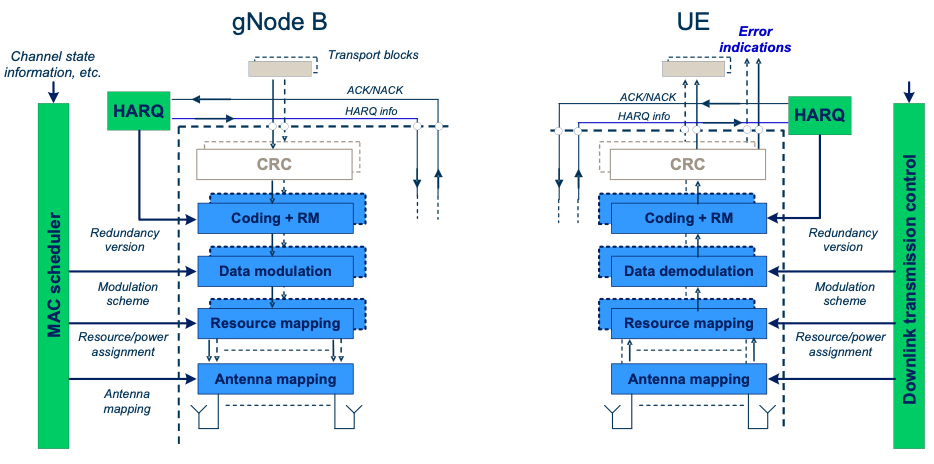
\includegraphics{PhysicalLayerModelForDLSCHTransmission}
	\caption{下行共享信道传输的物理层模型}
	\label{PhysicalLayerModelForDLSCHTransmission}
\end{figure}

该模型中包括以下步骤:
\begin{itemize}[leftmargin=2cm]
	\item 传递到物理层或从物理层传递的高层数据
	\item CRC 和传输块错误指示
	\item 向前纠错编码和速率匹配
	\item 数据调制
	\item 物理资源映射
	\item 多天线处理
	\item 支持 L1 控制和 HARQ 相关的信令
\end{itemize}

\subsubsection{广播信道}
广播信道(Broadcast CHannel, BCH)传输的物理层模型如图 \ref{PhysicalLayerModelForBCHTransmission} 所示。BCH 信道采用预定义的固定大小的传输格式,每 $80ms$ 有一个传输块。
\begin{figure}[!htbp]
	\centering
	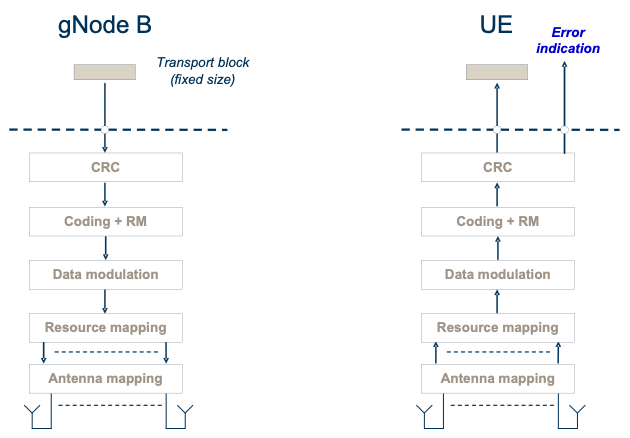
\includegraphics{PhysicalLayerModelForBCHTransmission}
	\caption{广播信道传输的物理层模型}
	\label{PhysicalLayerModelForBCHTransmission}
\end{figure}

该模型中包括以下步骤:
\begin{itemize}[leftmargin=2cm]
	\item 传递到物理层或从物理层传递的高层数据
	\item CRC 和传输块错误指示
	\item 向前纠错编码和速率匹配
	\item 数据调制
	\item 物理资源映射
	\item 多天线处理
\end{itemize}

\subsubsection{寻呼信道}
寻呼信道(Paging CHannel, PCH)传输的物理层模型如图 \ref{PhysicalLayerModelForPCHTransmission} 所示。PCH 承载在 PDSCH 上。图中蓝色部分显示的处理步骤表示它们可以通过高层配置。
\begin{figure}[!htbp]
	\centering
	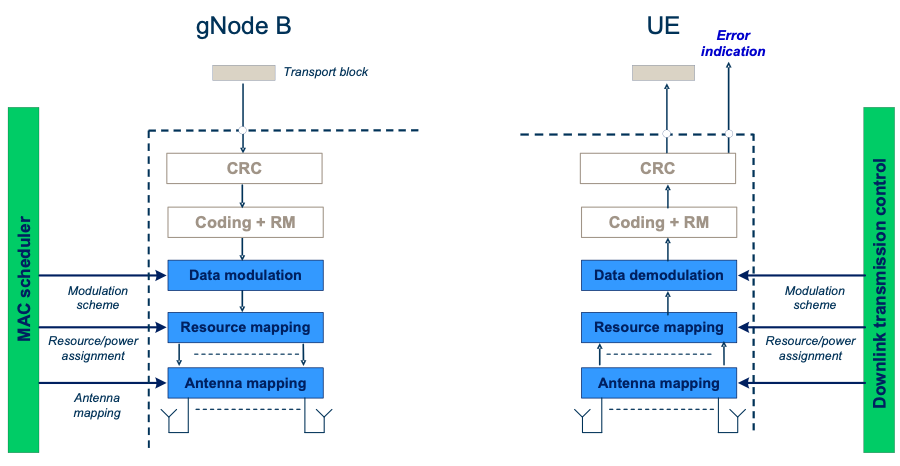
\includegraphics{PhysicalLayerModelForPCHTransmission}
	\caption{寻呼信道传输的物理层模型}
	\label{PhysicalLayerModelForPCHTransmission}
\end{figure}

该模型中包括以下步骤:
\begin{itemize}[leftmargin=2cm]
	\item 传递到物理层或从物理层传递的高层数据
	\item CRC 和传输块错误指示
	\item 向前纠错编码和速率匹配
	\item 数据调制
	\item 物理资源映射
	\item 多天线处理
\end{itemize}


\section{物理信道和物理信号的同时发送和接收}
根据 UE 的能力和服务要求,UE 需要同时发送和接收多个物理信道和物理信号。在接下来的上行链路和下行链路的描述中使用以下标记:
\begin{itemize}[leftmargin=2cm]
	\item $p$ 表示为 UE 配置的可以在其上发送物理信道的上行链路的载波数量
	\item $p^{'}$ 表示为 UE 配置的可以在其上发送 SRS 的上行链路的载波数量
	\item $q$ 表示为 UE 配置的下行链路的载波数量
	\item $j$ 表示为 UE 配置的小区组的数量
	\item $k$ 表示为 UE 配置的 PUCCH 组的数量
\end{itemize}

\subsection{上行链路}
为了便于描述,将物理信道或探测参考信号及其相关的传输信道定义为不同的“传输类型”,如表 \ref{UplinkTransmissionTypes} 所示。


\begin{table}[!htbp]
	\centering
	\resizebox{\textwidth}{!}{
		\begin{tabular}{|c|c|c|c|}
	\hline
	传输类型                          & 物理信道或探测参考信号                          & 相关传输信道                          & 注释                             \\ \hline
	A                             & PRACH                                & RACH                            & Note 1                         \\ \hline
	B                             & PUCCH                                & N/A                             &                                \\ \hline
	C                             & PUSCH                                & UL-SCH                          & Note 2                         \\ \hline
	D                             & SRS                                  & N/A                             &                                \\ \hline
	\multicolumn{4}{|l|}{\begin{tabular}[c]{@{}l@{}}Note 1: 这里的 RACH 指的是基于竞争的随机接入\\ Note 2: UCI 可以直接通过 PUSCH 发送,而不需要经过 UL-SCH\end{tabular}} \\ \hline
	\end{tabular}
	}

	\caption{上行链路传输类型}
	\label{UplinkTransmissionTypes}
\end{table}


基于 UE 能力的限制,UE 可以支持以下传输类型的组合。如表 \ref{UplinkTransmissionTypesCombinations}。

\begin{table}[!htbp]
	\centering
	\resizebox{\textwidth}{!}{
	\begin{tabular}{|p{0.5 \textwidth}<{\centering}|c|}
	\hline
	支持的组合 													& 注释  				\\ \hline 
	$j \times A$    											& Note 1  			\\ \hline
	$k \times B$  												& Note 2   		 	\\ \hline
	$p \times C$    											& Note 3, Note 4 	\\ \hline
	$p^{'} \times D$ 											& Note 3, Note 5    \\ \hline
	$\widetilde{j} \times A + \widetilde{k} \times B$  			& Note 6  			\\ \hline
	$\widetilde{j} \times A + \widetilde{p} \times C$  			& Note 6  			\\ \hline
	$\widetilde{j} \times A + \widetilde{p}^{'} \times D$    	& Note 6    		\\ \hline
	$\widehat{k} \times B + \widehat{p} \times C$            	& Note 8     		\\ \hline
	$\widetilde{k} \times B + \widetilde{p}^{'} \times D$    	& Note 7      		\\ \hline
	$\widetilde{p} \times C + \widetilde{p}^{'} \times D$    	& Note 7       		\\ \hline
	\multicolumn{2}{|l|}{
		\begin{tabularx}{\textwidth}{X}
		注1:组合中的小区组$j$的数量取决于 UE 的能力。\\ 
		注2:组合中的 PUCCH 组的数量 $k$ 取决于 UE 的能力。\\ 
		注3:组合中的载波数量 $p$ 和 $p^{'}$ 取决于UE的能力。\\ 
		注4:如果有一个 SUL 载波,则将只支持 $p-1$ 个 PUSCH。 \\ 
		注5:UE可以配置为 $p^{'}$,但 UE 的能力可能并不支持。\\ 
		注6:仅在带间CA的情况下才支持在 PUCCH(或PUSCH或SRS)同时进行PRACH,$\widetilde{j} \leq j$,$\widetilde{k} \leq k$,$\widetilde{p} \leq p$ 且 $\widetilde{p}^{'} \leq p^{'}$取决于配置,并取决于UE进行并行传输的能力。\\ 
		注7:仅在带间CA的情况下,才支持带有PUCCH(或PUSCH)的同时SRS, 其中$\widetilde{k} \leq k$,$\widetilde{p} \leq p$和$\widetilde{p}^{'} \leq p^{'}$取决于配置,并且取决于UE并行传输能力。\\ 
		注8:仅在配置了多个PUCCH组并且在不同的PUCCH组中发送各个PUCCH和PUSCH的情况下才支持同时PUCCH和PUSCH,且 $\widehat{k} < k$并且$\widehat{p} \leq p$。 $k$和$p$分别受UE功能支持的PUCCH组和UL载波数量的影响。 $\widehat{k}$和$\widehat{p}$取决于配置。
		\end{tabularx}}
		\\ \hline
	\end{tabular}}
	\caption{ 上行传输类型组合}
	\label{UplinkTransmissionTypesCombinations}
\end{table}

关于 UE 能力的更多内容可以参考 3GPP TS 38.306: "NR; User Equipment (UE) radio access capabilities"。

\newpage

\subsection{下行链路}
表 \ref{DownlinkReceptionTypes} 定义了 UE 在下行链路上可以接收的物理信道的类型。表 \ref{DownlinkReceptionTypesCombinations} 描述了 UE 可以在下行信道上同时接收物理信道的组合。UE 所能接收的信道类型的组合取决于其能力。UE 应该有能力根据 PDCCH 上的指示接收所有 TB 块。

\begin{table}[!htbp]
	\centering
	\resizebox{\textwidth}{!}{
	\begin{tabular}{|c|c|c|c|c|}
	\hline
	接收类型 & 物理信道          & RNTI                        & 相关传输信道 & 注释             \\ \hline
	A    & PBCH          & N/A                         & BCH    &                \\ \hline
	B    & PDCCH + PDSCH & SI-RNTI                     & DL-SCH & Note 1         \\ \hline
	C0   & PDCCH         & P-RNTI                      & N/A    & Note 1, Note 2 \\ \hline
	C1   & PDCCH + PDSCH & P-RNTI                      & PCH    & Note 1         \\ \hline
	D0   & PDCCH + PDSCH & RA-RNTI or Temporary C-RNTI & DL-SCH & Note 3         \\ \hline
	D1   & PDCCH + PDSCH & C-RNTI, CS-RNTI, MCS-C-RNTI & DL-SCH &                \\ \hline
	D2   & PDCCH         & C-RNTI, CS-RNTI, MCS-C-RNTI & DL-SCH &                \\ \hline
	E    & PDCCH         & C-RNTI                      & N/A    & Note 4         \\ \hline
	F0   & PDCCH         & Temporary C-RNTI            & UL-SCH &                \\ \hline
	F1   & PDCCH         & C-RNTI, CS-RNTI, MCS-C-RNTI & UL-SCH &                \\ \hline
	G    & PDCCH         & SFI-RNTI                    & N/A    &                \\ \hline
	H    & PDCCH         & INT-RNTI                    & N/A    &                \\ \hline
	J0   & PDCCH         & TPC-PUSCH-RNTI              & N/A    &                \\ \hline
	J1   & PDCCH         & TPC-PUCCH-RNTI              & N/A    &                \\ \hline
	J2   & PDCCH         & TPC-SRS-RNTI                & N/A    &                \\ \hline
	K    & PDCCH         & SP-CSI-RNTI                 & N/A    &                \\ \hline
	\multicolumn{5}{|l|}{\begin{tabular}[c]{@{}l@{}}
	Note 1: 这些信息仅从 PCell 上接收。\\ 
	Note 2: 在某些情况下,仅要求 UE 使用 P-RNTI 监控 DCI 中的短消息。\\ 
	Note 3: 这些信息可以从 PCell 上接收,也可以从 PSCell 上接收。\\ 
	Note 4: 对应于 PDCCH-ordered 的 PRACH。
	\end{tabular}} \\ 
	\hline
	\end{tabular}}
	\caption{下行链路接收类型}
	\label{DownlinkReceptionTypes}
\end{table}


\begin{table}[!htbp]
\centering
\resizebox{\textwidth}{!}{
	\begin{tabular}{|c|c|c|c|}
	\hline
	\multicolumn{3}{|c|}{支持的组合}                       & 注释     \\ \hline
	PCell                            & PSCell & SCell &        \\ \hline
	\multicolumn{4}{|l|}{1. RRC\_IDLE}                         \\ \hline
	A + (B and/or C1 and/or D0) + F0 &        &       & Note 1 \\ \hline
	\multicolumn{4}{|l|}{2. RRC\_INACTIVE}                     \\ \hline
	A + (B and/or C1 and/or D0) + F0 &        &       & Note 1 \\ \hline
	\multicolumn{4}{|l|}{3. RRC\_CONNECTED}                    \\ \hline
	\begin{tabular}[c]{@{}c@{}}A + C0 + (B and/or (D0 or (D1 + m*D2)))\\ + E + F0 + n*F1 + G + H + J0 + J1 + J2 + K\end{tabular} &
	  \begin{tabular}[c]{@{}c@{}}A + (D0 or (D1 + mD2)) + E + F0\\ + n*F1 + G + H + J0 + J1 + J2 + K\end{tabular} &
	  \begin{tabular}[c]{@{}c@{}}D1 + m*D2 + E + n*F1 + G \\ + H + J0 + J1 + J2 + K\end{tabular} &
	  \begin{tabular}[c]{@{}c@{}}Note 2, Note 3,\\ Note 4\end{tabular} \\ \hline
	\multicolumn{4}{|l|}{\begin{tabular}[c]{@{}l@{}}Note 1: UE 并不需要同时解码两个以上的 PDSCH。当 UE 接收到两个以上的 PDSCH 时,解码 PDSCH 的优先级取决于 UE 的实现。\\ Note 2: 当 PCell 在 FR1 频段时,UE 需要同时解码 SI-RNTI 加扰的 PDSCH 和 C-RNTI 加扰的 PDSCH。\\ Note 3: 所支持的组合取决于 UE 的能力:双链接、载波聚合、组 TPC 命令的接收、先占指示和动态 SFI 监视。\\ Note 4: 支持的组合中,$m \geq 0$ 和 $n \geq 0$,$m$ 和 $n$ 的值取决于 UE 的能力。\end{tabular}} \\ \hline
	\end{tabular}}
	\caption{下行链路接收类型组合}
	\label{DownlinkReceptionTypesCombinations}
\end{table}















\end{document}
